\naslov{Introduction}

\begin{definition}
  Let $\Gamma$ be a graph with vertex set $\Omega$ and adjacency relation
  $\sim$.
  A permutation $g$ of $\Omega$ is an \pojem{automorphism} or a \pojem{symmetry}
  of $\Gamma$ if for any $u, v \in \Omega$, $u$ and $v$ are adjacent if and only if $u^g$
  and $v^g$ are adjacent.
\end{definition}

\begin{example}
  Consider the symmetries of the Petersen graph.
  The standard picture is invariant under rotations by a multiple of $2 \pi /
  5$, and by the $5$ reflections along a line through the origin and an outer
  vertex.
  We can describe these symmetries by permutations (labeling the vertices as in
  figure~\ref{fig:sg-01-petersen}):
  \begin{itemize}
  \item A one-step rotation in the negative direction is represented by
	\[
	  \rho = (1\,2\,3\,4\,5) (6\,7\,8\,9\,10).
	\]
	Then the other rotations are $\rho^2$, $\rho^3$, $\rho^4$ and $\rho^5 =
	\id$.
  \item The reflection around the vertical line is
	\[
	  \tau = (1) (2\,5) (3\,5) (6) (7\,10) (8\,9).
	\]
	We have more reflections, for example
	\[
	  \tau' = (2) (1\,3) (4\,5) (7) (6\,8) (9\,10).
	\]
  \end{itemize}
  The orbits of all the above described permutations are $\{1,2,3,4,5\}$ and
  $\{6,7,8,9,10\}$.
  But there is another automorphism,
  \[
	\sigma =
	\begin{pmatrix}
	  1 & 2 & 3  & 4 & 5 & 6 & 7 & 8 & 9 & 10 \\
	  6 & 8 & 10 & 7 & 9 & 1 & 3 & 5 & 2 & 4
	\end{pmatrix}
	= (1\,6) (2\,8\,5\,9) (3\,10\,4\,7)
  \]
  This permutation is of degree $4$.
  It in interesting to consider $\sigma^2$; it must map the outer cycle to the
  inner cycle, and vice versa, so it must be in $\sk{\rho, \tau}$.
  We can compute $\sigma^2 = \tau$.
  As it turns out, there is no symmetry of this graph which maps the outer cycle
  to the inner cycle, and vice versa, but is of order $2$.

  Consider also the conjugation $\rho^\sigma = \sigma^{-1} \rho \sigma$.
  We can compute $\rho^\sigma = \rho^2$.
  Since $\tau^\sigma = (\sigma^2)^\sigma = \tau$,
  \[
	\sk{\tau, \rho}^\sigma = \sk{\tau^\sigma, \rho^\sigma} = \sk{\tau, \rho^2}
	= \sk{\tau, \rho}
  \]
  and we have $\sk{\tau, \rho} \trianglelefteq H := \sk{\rho, \tau, \sigma}$ and
  $\sigma^2 \in \sk{\tau, \rho}$.
  So $\abs{H} = 2 \abs{\sk{\tau, \rho}} = 20$.
  But there are more automorphisms.

  We can relabel the vertices if the Petersen graph with elements of the set
  $\binom{[5]}{2}$ (note that for a set $S$, $\binom{S}{k}$ denotes the set of
  all $k$-subsets of $S$), as in figure~\ref{fig:sg-01-petersen-relabeled}.
  Note that $U, V \in \binom{[5]}{2}$ are connected if and only if they are
  disjoint (as sets).
  For any permutation $g \in S_5$, we can find a permutation $\alpha_g \in \Sym
  \binom{[5]}{2}$ which permutes the pairs by permuting their elements as $g$
  would.
  So there are at least $\abs{S_5} = 120$ automorphisms of the Petersen graph.
  Note that $g \mapsto \alpha_g$ is a group homomorphism.
\end{example}

\begin{figure*}[h!]
  \centering
  \begin{subfigure}{0.4\linewidth}
	\centering
	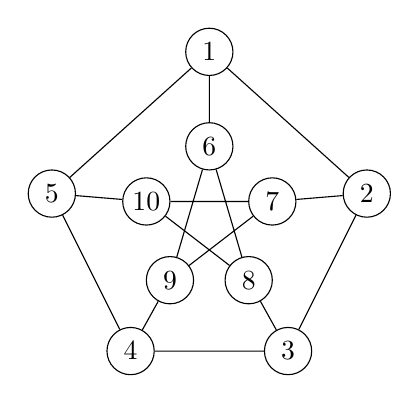
\begin{tikzpicture}
	  \node[draw,circle,minimum size=0.6cm,inner sep=0pt] (1) at (0,3.8) {1};
	  \node[draw,circle,minimum size=0.6cm,inner sep=0pt] (2) at (2,2) {2};
	  \node[draw,circle,minimum size=0.6cm,inner sep=0pt] (3) at (1,0) {3};
	  \node[draw,circle,minimum size=0.6cm,inner sep=0pt] (4) at (-1,0) {4};
	  \node[draw,circle,minimum size=0.6cm,inner sep=0pt] (5) at (-2,2) {5};
	  \node[draw,circle,minimum size=0.6cm,inner sep=0pt] (6) at (0,2.6) {6};
	  \node[draw,circle,minimum size=0.6cm,inner sep=0pt] (7) at (0.8,1.9) {7};
	  \node[draw,circle,minimum size=0.6cm,inner sep=0pt] (8) at (0.5,0.9) {8};
	  \node[draw,circle,minimum size=0.6cm,inner sep=0pt] (9) at (-0.5,0.9) {9};
	  \node[draw,circle,minimum size=0.6cm,inner sep=0pt] (10) at (-0.8,1.9) {10};

	  \draw (1) -- (2) -- (3) -- (4) -- (5) -- (1);
	  \draw (1) -- (6) (2) -- (7) (3) -- (8) (4) -- (9) (5) -- (10);
	  \draw (6) -- (8) -- (10) -- (7) -- (9) -- (6);
	\end{tikzpicture}
	\caption{The first labeling.}%
	\label{fig:sg-01-petersen}
  \end{subfigure}
  \begin{subfigure}{0.4\linewidth}
	\centering
	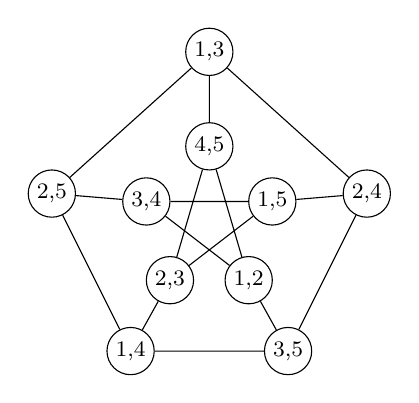
\begin{tikzpicture}
	  \node[draw,circle,minimum size=0.6cm,inner sep=0pt] (1) at (0,3.8) {\footnotesize 1,3};
	  \node[draw,circle,minimum size=0.6cm,inner sep=0pt] (2) at (2,2) {\footnotesize 2,4};
	  \node[draw,circle,minimum size=0.6cm,inner sep=0pt] (3) at (1,0) {\footnotesize 3,5};
	  \node[draw,circle,minimum size=0.6cm,inner sep=0pt] (4) at (-1,0) {\footnotesize 1,4};
	  \node[draw,circle,minimum size=0.6cm,inner sep=0pt] (5) at (-2,2) {\footnotesize 2,5};
	  \node[draw,circle,minimum size=0.6cm,inner sep=0pt] (6) at (0,2.6) {\footnotesize 4,5};
	  \node[draw,circle,minimum size=0.6cm,inner sep=0pt] (7) at (0.8,1.9) {\footnotesize 1,5};
	  \node[draw,circle,minimum size=0.6cm,inner sep=0pt] (8) at (0.5,0.9) {\footnotesize 1,2};
	  \node[draw,circle,minimum size=0.6cm,inner sep=0pt] (9) at (-0.5,0.9) {\footnotesize 2,3};
	  \node[draw,circle,minimum size=0.6cm,inner sep=0pt] (10) at (-0.8,1.9) {\footnotesize 3,4};

	  \draw (1) -- (2) -- (3) -- (4) -- (5) -- (1);
	  \draw (1) -- (6) (2) -- (7) (3) -- (8) (4) -- (9) (5) -- (10);
	  \draw (6) -- (8) -- (10) -- (7) -- (9) -- (6);
	\end{tikzpicture}
	\caption{The second ordering}%
	\label{fig:sg-01-petersen-relabeled}
  \end{subfigure}
  \caption{The Petersen graph}
\end{figure*}

\begin{definition}
  Let $\Omega$ be a nonempty finite set.
  A \pojem{permutation} on $\Omega$ is a bijection $\Omega \to \Omega$.
  We denote the set of all permutations of $\Omega$ with $\Sym \Omega$, or
  $S_n$, if $\Omega = [n]$.
\end{definition}

\begin{definition}
  If $g \in \Sym \Omega$ and $\omega \in \Omega$, then $\omega^g = g(\omega)$
  denotes the application of $g$ on $\omega$.
\end{definition}

\begin{definition}
  The composition of two permutations $g, h \in \Sym \Omega$ is defined as the
  permutation which acts as
  \[
	g \circ h: \omega \to g(h(\omega)) = {(\omega^h)}^g.
  \]
\end{definition}

We introduce the inverse composition as our product operation on $\Sym \Omega$,
defined as
\[
  gh = h \circ g.
\]
Then $\omega^{(g h)} = {(\omega^g)}^h =: \omega^{gh}$.
Note that both $(\Sym \Omega, \circ)$ and $(\Sym \Omega, \cdot)$ are groups, and
they are different groups, but they are isomorphic.

\begin{definition}
  We denote the set of all transpositions of $\Omega$ with $T_\Omega$.
\end{definition}

\begin{remark}
  Note that $\sk{T_\Omega} = \Sym \Omega$.
\end{remark}

\begin{definition}
  Denote by $\Alt \Omega$ the set of all even permutations of $\Omega$.
\end{definition}

\begin{remark}
  This is an index-$2$ normal subgroup in $\Sym \Omega$.
\end{remark}

\begin{definition}
  The \pojem{cyclic} group of order $n$ is $\Cyc(n) =
  \sk{(1\,2\,3\,\ldots\,n)} \le S_n$.
\end{definition}

\begin{definition}
  The \pojem{dihedral} group of order $n$ is
  \[
	\Dih(n) =
	\begin{cases}
	  \sk{(1\,2\,3\,\ldots\,n), (1) (2,n) (3,n-1) \ldots
	  (\frac{n}{2},\frac{n+2}{2})} & \text{$n$ even} \\
	  \sk{ (1\,2\,3\,\ldots\,n), (1) (2,n-1) \ldots
	  (\frac{n+1}{2},\frac{n+3}{2}) } & \text{$n$ odd}
	\end{cases}
  \]
  as a subgroup of $S_n$.
\end{definition}

\begin{remark}
  This is the automorphism group of a cyclic graph on $n$ vertices.
\end{remark}

\begin{definition}
  Let $G$ be an abstract group and $\Omega$ a set.
  A \pojem{group action} is a group homomorphism $\rho: G \to \Sym \Omega$.
\end{definition}

\begin{remark}
  We often write $\omega^g$ when we really mean $\omega^{\rho(g)}$.
\end{remark}

\begin{remark}
  As a shorthand, we can write $\rho(g) = g^\Omega$, and $G^\Omega = \rho(G) =
  \{ g^\Omega \such g \in G \}$.
\end{remark}

\begin{definition}
  An action is \pojem{faithful} if the kernel of the action is trivial.
\end{definition}

\begin{remark}
  Note that $G^\Omega = \im \rho \cong G / \jedro \rho$.
\end{remark}

\begin{remark}
  Any faithful action is an isomorphism $G \to G^\Omega$, so we may view $G$ as
  a subgroup in $\Sym \Omega$.
  So $G$ becomes a permutation group.
\end{remark}